\section{Transportschicht}

\paragraph{Internet-Protokollstack}
\begin{items}
  \item Anwendungsschicht
  \item \textbf{Transportschicht}
  \item Vermittlungsschicht
  \item Sicherungsschicht
  \item Physikalische Schicht
\end{items}

\paragraph{Transportschicht --- Ziel}
\begin{items}
  \item \emph{Verbergen von Transportdetails vor höheren Schichten} \\*
    - Fehlercharakteristika \\*
    - genutzte Technologien \\*
    - \dots
  \item \emph{Bereitstellung von Transportdiensten} \\*
    \( \leadsto \) \textbf{Nutzer-zu-Nutzer-Kommunikation}
\end{items}

\paragraph{Transportprotokolle --- Prinzip}
\begin{items}
  \item Transportprotokoll läuft auf Endsystemen
  \item \textbf{Sender}: \\*
    - \emph{Segmentieren} von Anwendungsnachrichten \\*
    - \emph{Weiterleiten} an Vermittlungsschicht
  \item \textbf{Empfänger}: \\*
    - \emph{Reassemblieren} der Segmente in Nachrichten \\*
    - \emph{Weiterleiten} an Anwendungsschicht
\end{items}

\paragraph{Transportschicht --- Transportdienste}
\begin{items}
  \item \textbf{UDP} (\emph{user datagram protocol}): \\*
    bietet verbindungslosen, \textbf{unzuverlässigen} Transportdienst
  \item \textbf{TCP} (\emph{transmission control protocol}): \\*
    bietet verbindungsorientierten, \textbf{zuverlässigen} Transportdienst
\end{items}

\paragraph{Transportdienst --- unzuverlässig vs zuverlässig}
\begin{items}
  \item \textbf{Unzuverlässig}: \\*
    - unklar, wieviel der gesendeten Daten heil ankommt \\*
    - keine Fehlermaßnahmen
  \item \textbf{Zuverlässig}: \\*
    - \emph{Korrektheit}, \emph{Vollständigkeit}, \emph{Reihenfolge} garantiert richtig \\*
    - keine Duplikate \\*
    - keine Phantom-Pakete \\*
    - Fehlermaßnahmen existieren
\end{items}

\paragraph{Schicht vs Dienst}
\begin{items}
  \item \textbf{Schicht}: Abstraktion \\*
  \item \textbf{Dienst}: Bündelung zusammengehöriger Funktionen \\*
    - Höhere Schicht nutzt Dienst darunterliegender Schicht \\*
    - Dienste werden an Dienstzugangspunkt einer Schicht bereitgestellt
\end{items}

\paragraph{Port}
\begin{items}
  \item = \emph{Adressen der Transportschicht}
  \item Unstrukturierte Nummer (16 Bit), 0 bis 65535
  \item \textbf{Well known ports}: viele Portnummern unter 1024 für häufig benutzte Anwendungen (Telnet, HTTP, \dots) reserviert
\end{items}

\paragraph{IP-Adressen}
\begin{items}
  \item = \emph{Adressen der Vermittlungsschicht}
  \item \textbf{IPv4}: 32 Bit (z.B. 207.142.131.235)
  \item \textbf{IPv6}: 128 Bit (z.B. 2001:0db8:85a3:08d3:1319:8a2e:0370:7344)
  \item \( \leadsto \) Internetweite Adressierung eines Anwendungsprozesses: IP-Adresse + Port
\end{items}

\newpage

\paragraph{UDP}
\begin{items}
  \item RFC768 --- \emph{sehr einfaches Transportprotokoll mit sehr geringem Overhead}
  \item \textbf{Eigenschaften}: \\*
    - (De-) Multiplexen von Segmenten für Prozesse \\*
    - \emph{Prüfsumme} für Bitfehler \\*
    - \emph{verbindungslos} \\*
    - \emph{best effort}: keine Zusagen über Auslieferung bei Empfänger \\*
    - \emph{Unreguliertes Senden}: kann Daten so schnell senden wie von Anwendung geliefert \\* \phantom{-} und von Netz abgenommen \\*
    - \emph{keine Verbindungsaufbauphase}: sofortiges Senden \( \leadsto \) keine weitere Verzögerung \\*
    - \emph{kein Verbindungszustand}: keine Verbindungsinformationen im Endsystem \\* \phantom{-} \( \leadsto \) skaliert z.B. für Server besser
  \item \textbf{Verwendung}: \\*
    - \textbf{Multimedia} \\*
    - \textbf{DNS}
\end{items}
\begin{figure}[H]\centering\label{UDPAufbau}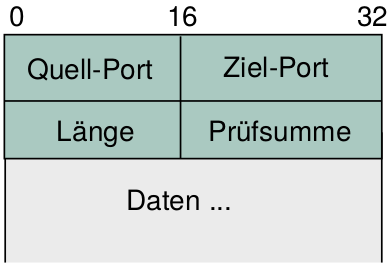
\includegraphics[width=0.2\textwidth]{UDPAufbau}\end{figure}

\paragraph{Protokollmechanismen}
\begin{items}
  \item \textbf{Ziel}: \emph{Datenaustausch zwischen Anwendungen/Geräten ermöglichen}
  \item \( \leadsto \) Festlegen von Formaten + Regeln für Datenaustausch nötig
  \item \textbf{Problem}: Fehler bei Datenübertragung möglich
\end{items}

\paragraph{Bitfehler}
\begin{items}
  \item \emph{Verfälschung von Bits während dem Datentransport}
  \item \textbf{Ursachen}: \\*
    - Dämpfung Übertragungssignal \\*
    - Übersprechen \\*
    - Synchronisationsverlust \\*
    - \dots
  \item \textbf{Einzelbitfehler}: ein \emph{einzelnes} Bit fehlerhaft
  \item \textbf{Bündelfehler}: mehrere aufeinanderfolgende Bits fehlerhaft
\end{items}

\paragraph{Paketfehler}
\begin{items}
  \item \textbf{Fehlerarten}: \\*
    - Verlust \\*
    - Duplizierung \\*
    - Phantom-Paket \\*
    - Reihenfolgenvertauschung
  \item \textbf{Fehlerursachen}: \\*
    - Zwischennetzüberlastung \\*
    - Unterschiedliche Wege durch Netz \\*
    - Verfrühte Datenwiederholung \\*
    - \dots
\end{items}

\paragraph{Fehler --- Häufigkeit und Auswirkungen}
\begin{items}
  \item \textbf{Bitfehlerrate}: Maß für Fehlerhäufigkeit \\*
   \( \text{Bitfehlerrate} = \tfrac{\text{Summe gestörter Bits}}{\text{Summe übertragener Bits}} \)
  \item \textbf{Fehlerauswirkungen}: 20ms Störung in \\*
    - Telex (50bit/s \( \leadsto \) Bitdauer 20ms): 1 Bit fehlerhaft (Einzelbitfehler) \\*
    - Gigabit-Ethernet (1Gbit/s \( \leadsto \) Bitdauer 1ns): 20MBit fehlerhaft (Bündelfehler)
\end{items}

\paragraph{Fehler --- Gegenmaßnahmen}
\begin{items}
  \item \textbf{Fehlererkennung} (\emph{error detecting code}, EDC) \\*
    - Redundanz zu Daten hinzufügen \\*
    - Ausreichend stark unterschiedliche Codewörter verwenden
  \item \textbf{Fehlerkorrektur} (\emph{forward error correction}, FEC) \\*
    - Fehler mittels Redundanz korrigieren
  \item \textbf{Wiederholungsaufforderung} (\emph{automatic repeat request}, ARQ) \\*
    - Empfänger teilt Sender Ergebnis der Fehlerkorrektur mit
\end{items}

\paragraph{Fehlerkontrolle --- Bitfehler}
\begin{items}
  \item \textbf{Problem}: Wie Bitfehler erkennen?
  \item \textbf{Ansatz}: Hinzufügen von Redundanz
  \item \emph{Paritätsprüfung}: bekannt
\end{items}

\paragraph{Bitfehler --- Internet-Prüfsumme}
\begin{items}
  \item \textbf{Prinzip}: Aufaddieren aller übertragenen Wörter (16 Bit, als Integer interpretiert) \\* 
    \( \leadsto \) Prüfsumme
  \item \textbf{Nachteil}: Falsche Reihenfolge kann nicht erkannt werden
\end{items}
\begin{figure}[H]\centering\label{Internetpruefsumme}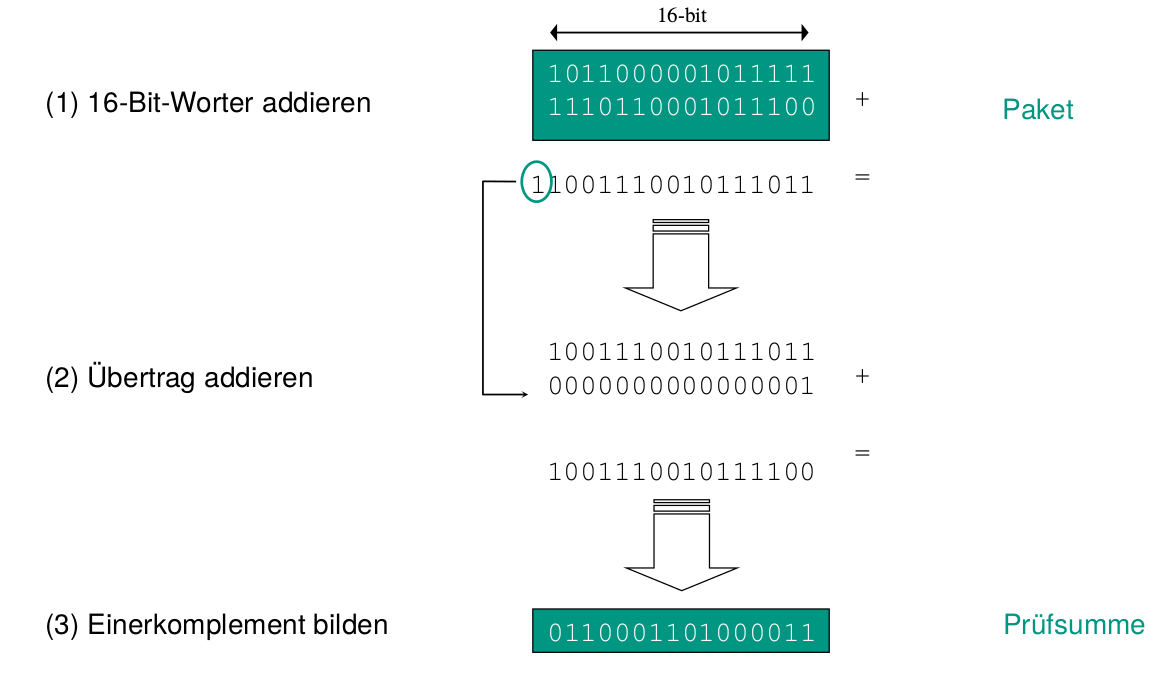
\includegraphics[width=0.33\textwidth]{Internetpruefsumme}\end{figure}

\paragraph{Bitfehler --- UDP-Prüfsumme}
\begin{items}
  \item \textbf{Sender}: \\*
    - UDP-Segment + -Kopf wird als Folge von 16 Bit-Wörtern aufgefasst \\*
    - Prüfsumme berechnen und in UDP-Kopf einfügen
  \item \textbf{Empfänger}: \\*
    - Prüfsumme des UDP-Segments berechnen
    - Prüfsummen vergleichen
\end{items}

\paragraph{Fehlerkontrolle --- Paketfehler}
\begin{items}
  \item \textbf{Erkennung}: \\*
    - Sequenznummern (\emph{sequence number}) \\*
    - Zeitgeber (\emph{timer})
  \item \textbf{Behebung}: \\*
    - Quittungen (\emph{acknowledgements}) \\*
    - Sendewiederholungen (\emph{retransmissions})
\end{items}

\paragraph{Paketfehler --- Sequenznummern}
\begin{items}
  \item \textbf{Problem}: Empfänger weiß nicht, ob Pakete richtig (Reihenfolge, Duplikate, Vollständigkeit) angekommen sind
  \item \textbf{Prinzip}: Pakete werden durchnummeriert
\end{items}

\paragraph{Paketfehler --- Quittungen}
\begin{items}
  \item \textbf{Problem}: Sender erfährt nicht, ob Paket nicht (korrekt) angekommen ist
  \item \textbf{Prinzip}: \\*
    - Empfänger informiert Sender über Erhalt \\*
      \phantom{-} \( \leadsto \) \emph{Acknowledgement} (ACK)
  \item \textbf{Varianten}: \\*
    - \emph{positive Quittung}: Empfänger sagt Sender, dass er Daten erhalten hat (ACK) \\*
    - \emph{negative Quittung}: Empfänger sagt Sender, dass er Daten \emph{nicht} erhalten hat (NACK) \\*
    - \emph{selektive Quittung}: Quittiert einzelnes Paket --- z.B. bei Verlustvermutung (NACK) \\*
    - \emph{kumulative Quittung}: Quittiert Paketmenge --- z.B. alle Pakete bis bestimmte \\* \phantom{-} \phantom{-} Sequenznummer sind ok
\end{items}

\paragraph{Paketfehler --- Zeitgeber}
\begin{items}
  \item \textbf{Problem}: Sender merkt nicht, wenn Paket nicht angekommen ist
  \item \textbf{Prinzip}: Durch zeitliche Obergrenze wird \emph{vermutet}, dass Paket nicht angekommen ist \\* \( \leadsto \) \emph{Sendewiederholung}
\end{items}

\paragraph{Sendewiederholung --- ARQ}
\begin{items}
  \item = \emph{automatic repeat request}
  \item Grundlegende Sendewiederholungsvariante
  \item \textbf{Varianten}: \\*
    - Wann werden Quittungen versendet? \\*
    - Wann wird eine Sendung wiederholt?
\end{items}

\paragraph{Sendewiederholung --- Stop-and-Wait}
\begin{items}
  \item = einfaches ARQ-Verfahren
  \item \textbf{Prinzip}: \\*
    - Sender wartet auf Quittung für gesendetes Paket \\*
    - Erst \emph{nach} Quittungserhalt wird nächstes Paket gesendet \\*
    - keine Quittung \( \leadsto \) Sendewiederholung \\*
    - Wartezeit durch Zeitgeber geregelt
\end{items}

\paragraph{Stop-and-Wait --- Sequenznummern}
\begin{items}
  \item \textbf{Problem}: Empfänger kann Paket doppelt erhalten (nicht erkennbar)
  \item \textbf{Prinzip}: Pakete werden mit Sequenznummern versehen (für Stop-and-Wait reicht 1 Bit)
  \item \textbf{Auslastung}: \( U = \tfrac{1}{1+2a} \) (mit \( a = \tfrac{t_a}{t_s} \))
\end{items}

\paragraph{Bandbreitenverzögerungsprodukt}
\begin{items}
  \item \( \eqqcolon \tfrac{m}{v}r \) (Länge \( m \), Ausbreitungsgeschwindigkeit \( v \), Datenrate \( r \))
  \item = \textbf{Speicherkapazität des Mediums}
\end{items}

\paragraph{Sendewiederholung --- Go-Back-N ARQ}
\begin{items}
  \item \textbf{Zeil}: Leistungsfähigkeit von Stop-and-Wait erhöhen
  \item \textbf{Prinzip}: \\*
    - Sender sendet mehrere Pakete bis Quittungspflicht \\*
    - begrenzte Anzahl an nicht quittierten Paketen (durch \textbf{Fenster} (\emph{window}) begrenzt) \\*
    - Quittierung durch kumulative Quittungen
  \item \textbf{Fehlerfall}: \\*
    1. Empfänger empfängt fehlerhaftes Paket \\*
    2. Empfänger verwirft alle nachfolgenden Pakete
    3. Sender wartet auf Ablauf des Zeitgebers \\*
    4. Sender wiederholt alle nicht quittierten Pakete
  \item \textbf{Fragen}: \\*
    - Wo müssen Pakete gepuffert werden? \\*
    - Wieviele Pakete müssen gepuffert werden?
  \item \textbf{Auslastung}: \( U = \begin{cases}
    1 & W \geq 1+2a \\
    \tfrac{W}{1+2a} & \text{sonst}
  \end{cases} \)
\end{items}

\paragraph{Sendewiederholung --- Selective Repeat ARQ}
\begin{items}
  \item \textbf{Ziel}: \\*
    - Auslastung von Stop-and-Wait erhöhen \\*
    - Datenaufkommen von Go-Back-N reduzieren
  \item \textbf{Prinzip}: Wie Go-Back-N, Empfänger quittiert selektiv
  \item \textbf{Fehlerfall}: \\*
    1. Empfänger bestätigt nachfolgende, korrekt empfangene Pakete \\*
    2. Sender wiederholt nur nicht korrekt empfangene Pakete
  \item \textbf{Fragen}: \\*
    - Wo müssen Pakete gepuffert werden? \\*
    - Wieviele Pakete müssen gepuffert werden? \\*
    - Vor-/Nachteile von Go-Back-N und Selective Repeat
\end{items}

\paragraph{Sendewiederholung --- Selective Repeat vs. Selective Reject}
\begin{items}
  \item \textbf{Selective Repeat}: \\*
    - Fehlerhaftes Paket wird nicht bestätigt \\*
    - Sender wartet auf Timeout
  \item \textbf{Selective Reject}: \\*
    - Empfänger versendet für fehlerhaftes Paket negative Quittung \\*
    - Sender wiederholt sofort und wartet nicht auf Timeout
\end{items}

\paragraph{Paketfehler --- Vorwärtsfehlerkorrektur}
\begin{items}
  \item \textbf{Ziel}: Empfänger muss nur drei von vier Paketen korrekt empfangen um fehlendes Paket rekonstruieren zu können
  \item \textbf{Prinzip}: XOR-Verknüpfung der drei Pakete \( \leadsto \) fehlendes Paket
\end{items}

\paragraph{Flusskontrolle}
\begin{items}
  \item \textbf{Problem}: \\*
    - \emph{Überlastung} von Empfänger durch Sender \( \leadsto \) Datenverlust
    - Sendet muss Empfangspuffergröße berücksichtigen
  \item \textbf{Anforderungen}: \\*
    - einfach \\*
    - möglichst wenig Netzressourcen nutzen \\*
    - fair \\*
    - stabil
\end{items}

\paragraph{Flusskontrolle --- Halt-und-Weiter}
\begin{items}
  \item \textbf{Prinzip}: \\*
    - Empfänger kommt nicht mehr mit \( \leadsto \) \code{halt}-Signal \\*
    - Empfänger wieder verfügbar \( \leadsto \) \code{weiter}-Signal
  \item \textbf{Bewertung}: \\*
    - nut auf Vollduplex verwendbar \\*
    - nicht effektiv bei hohen Verzögerungen \\*
    - Probleme bei Verlust der \code{halt}-Meldung
  \item \textbf{Beispiele}: \\*
    - Fast- + Gigabit-Ethernet
\end{items}

\paragraph{Flusskontrolle --- Stop-and-Wait}
\begin{items}
  \item \textbf{Prinzip}: \\*
    - Empfänger sendet Quittung erst, wenn er wieder kann \\*
    - Sender wird durch Zurückhalten gebremst
  \item \textbf{Problem}: \\*
    - Sender kann nicht zwischen Datenverlust und Überlastung unterscheiden
\end{items}

\paragraph{Flusskontrolle --- Kreditbasiert}
\begin{items}
  \item \textbf{Prinzip}: \\*
    - Sender kann höchstens \( n \) Pakete unquittiert senden \\*
    - \( n \) = Pufferkapazität des Senders \( \Rightarrow \) \textbf{Sendekredit} \\*
    - Alternativbezeichnung: Fenster (\emph{sliding window}) \\*
    - Fenster wird durch korrekte positive Quittung weitergeschaltet \\*
    - Empfänger kann Kredit bestimmen (z.B. in TCP)
\end{items}

\paragraph{TCP --- Prinzip}
\begin{items}
  \item \emph{Erhält Bytestrom von Anwendung, übergibt TCP-Segmente an IP}
  \item \textbf{Problem}: Wie Bytestrom in TCP-Segmente schnippeln?
  \item \textbf{Implementierung}: \\*
    - MSS (\emph{maximum segment size}): Anwendungsdatenlänge (z.B. 1460 Byte) \\*
    - Push (\code{PSH} in TCP-Segmentkopf): Sender verlangt sofortiges Versenden der Daten \\*
    - Zeitgeber: nach inaktivem Zeitintervall werden vorhandene Daten gesendet
  \item \textbf{Fehlerkontrolle}: Sequenznr., Prüfsumme, Quittierungen, Sendewiederholungen
  \item \textbf{Sequenznummern}: pro Byte, nicht pro Segment (erstes Byte in Segment, initiale Sequenznummer von Endsystem \emph{zufällig} gewählt)
\end{items}
\begin{figure}[H]\centering\label{TCPAufbau}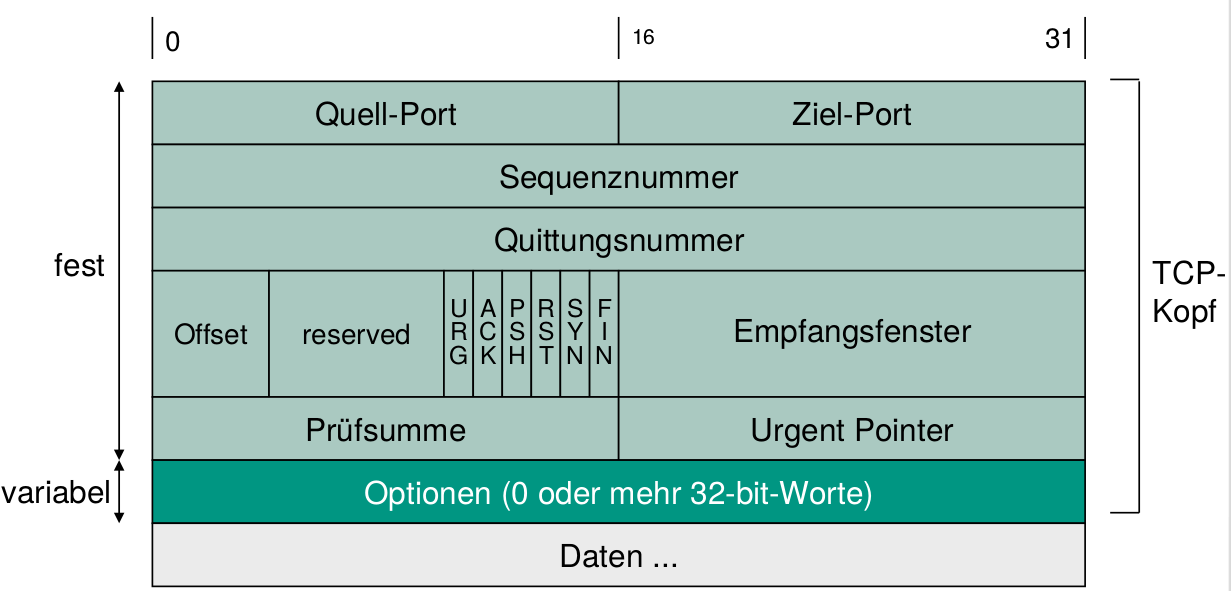
\includegraphics[width=0.33\textwidth]{TCPAufbau}\end{figure}

\paragraph{TCP --- Felder}
\begin{items}
  \item \textbf{Quell-/Ziel-Port}: Identifizieren Verbindungsendpunkte
  \item \textbf{Sequenznummer}: gemessen in Byte, nicht pro Segment
  \item \textbf{Quittung}: nächste von Empfänger erwartete Sequenznummer
  \item \textbf{Offset}: Anzahl 32 Bit-Wörter in TCP-Kopf
  \item \textbf{URG}: 1, falls \emph{urgent pointer} verwendet wird (idR leer)
  \item \textbf{SYN}: Wird bei Verbindungsaufbau verwendet, um \emph{connection request} oder \emph{connection confirmation} anzuzeigen
  \item \textbf{ACK}: unterscheidet bei gesetztem SYN-Bit zwischen Request und Confirmation; signalisiert Gültigkeit von Quittungsfeld
  \item \textbf{FIN}: gibt an, dass Sender nichts mehr senden möchte
  \item \textbf{RST}: Verbindung zurücksetzen
  \item \textbf{PSH}: übergebene Daten sollen sofort weitergeleitet werden (idR leer)
  \item \textbf{Empfangsfenster}: für Flusskontrolle
  \item \textbf{Prüfsumme}: Prüfsumme über TCP-Kopf, Daten und Pseudoheader
  \item \textbf{Urgent-Zeiger}: relativer Zeiger auf wichtige Daten
  \item \textbf{Optionen-Feld}: kann Optionen variabler Länge aufnehmen
\end{items}

\paragraph{TCP --- Flusskontrolle}
\begin{items}
  \item \textbf{Ziel}: Empfängerüberlastung vermeidne
  \item \textbf{Prinzip}: \\*
    - \emph{Empfänger}: reserviert Pufferplatz pro Verbindung (explizite Kreditvergabe) \\*
    \phantom{-} \( \cdot \) \code{RcvBuffer}: gesamter Pufferplatz (default 4096 Byte) \\*
    \phantom{-} \( \cdot \) \code{RcvWindow}: freier Pufferplatz (Empfangsfenster) \\*
    \phantom{-} \( \cdot \) Sender sendet nicht mehr unbestätigt als in \code{RcvWindow} passt
\end{items}
\begin{figure}[H]\centering\label{TCPBuffer}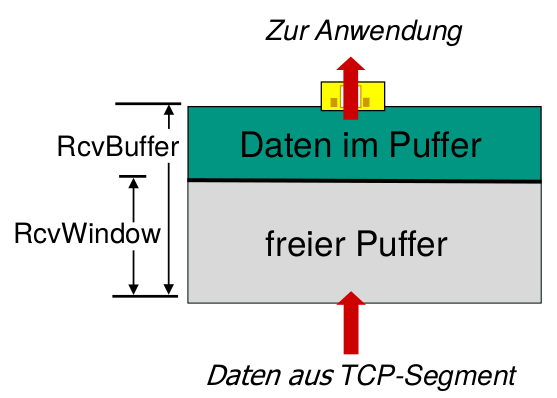
\includegraphics[width=0.2\textwidth]{TCPBuffer}\end{figure}

\paragraph{Verbindungen --- verbindungslos vs. verbindungsorientiert}
\begin{items}
  \item \textbf{Verbindungslos}: \\*
    - Daten werden ohne vorherigen Handshake gesendet \\*
    - \emph{Vorteil}: schnelle Datenversendung möglich \\*
    - \emph{Nachteil}: kein Feedback, keine Bestätigung
  \item \textbf{Verbindungsorientiert}: \\*
    - Verbindungsaufbau vor Datenaustausch, Verbindungsabbau danach \\*
    - \emph{Vorteil}: Kommunikationsparameter können ausgehandelt werden \\*
    - \emph{Nachteile}: Verzögerter Datenaustausch, Overhead ggf größer als Daten
\end{items}

\paragraph{TCP --- Zusammenspiel mit HTTP}
\begin{figure}[H]\centering\label{TCPHTTP}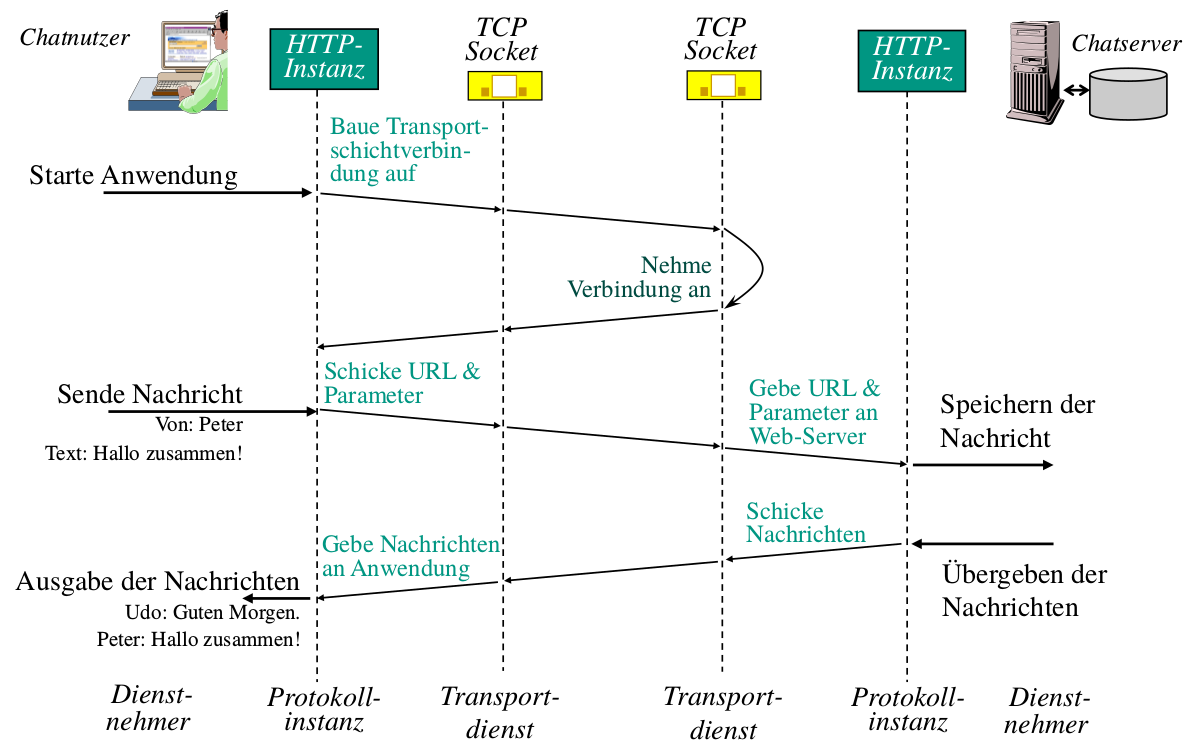
\includegraphics[width=0.4\textwidth]{TCPHTTP}\end{figure}

\paragraph{Staukontrolle}
\begin{items}
  \item \textbf{Ziel}: Netzüberlastungssituationen vermeidne
  \item \textbf{Prinzip}: \\*
    - Staukontrollfenster (\emph{congestion window}, CWnd) beim Sender beeinflusst \\* \phantom{-} \phantom{\( \cdot \)} maximal zu sendende Datenmenge: \\* \phantom{-} \( \cdot \) \( \text{LastByteSent} - \text{LastByteAcked} \leq \text{min} \{ \text{CWnd}, \text{RcvWindow} \} \) \\*
    - Schwellenwert (SSTresh) \\*
  \item \textbf{Stauerkennung}: \\*
    - Nutzung von Zeitgebern \\*
    - Vermutung einer Stausituation bei ausbleibender Quittung \\*
  \item \textbf{Staubehebung}: \\*
    - Reduktion von \code{CWnd} \\*
    - Langsames Erhöhen von \code{CWnd} \( \leadsto \) herantasten an Netzkapazität
\end{items}

\paragraph{Staukontrolle --- TCP}
\begin{items}
  \item \textbf{Start}: \code{CWnd} = 1 \code{MSS} (\emph{maximum segment size})
  \item \textbf{Slow-Start}, falls \code{CWnd} \( \leq \) \code{SSTresh} \& Quittungen rechtzeitig da \\*
    - \emph{Exponentielles} Erhöhen \code{CWnd} (\code{CWnd} += 1 bei jeder empfangenen Quittung)
  \item \textbf{Congestion Avoidance}, falls \code{CWnd} > \code{SSTresh} \& Quittungen rechtzeitig da \\*
    - \emph{Lineares} Erhöhen \code{CWnd} (\code{CWnd} += \( \tfrac{1}{\text{\code{CWnd}}} \) bei jeder empfangenen Quittung)
  \item \textbf{Congestion}, falls Quittung nicht rechtzeitig da \\*
    - Stau vermutet \\*
    - \( \text{\code{SSTresh}} = \text{max}(\tfrac{\text{FlightSize}}{2}, 2*\text{MSS}) \) (FlightSize = unquittierte, gesendete Daten) \\*
    - \code{CWnd} zurücksetzen (neue Slow-Start-Phase): \code{CWnd} = 1 \code{MSS}
\end{items}
\begin{figure}[H]\centering\label{TCPStaukontrolle}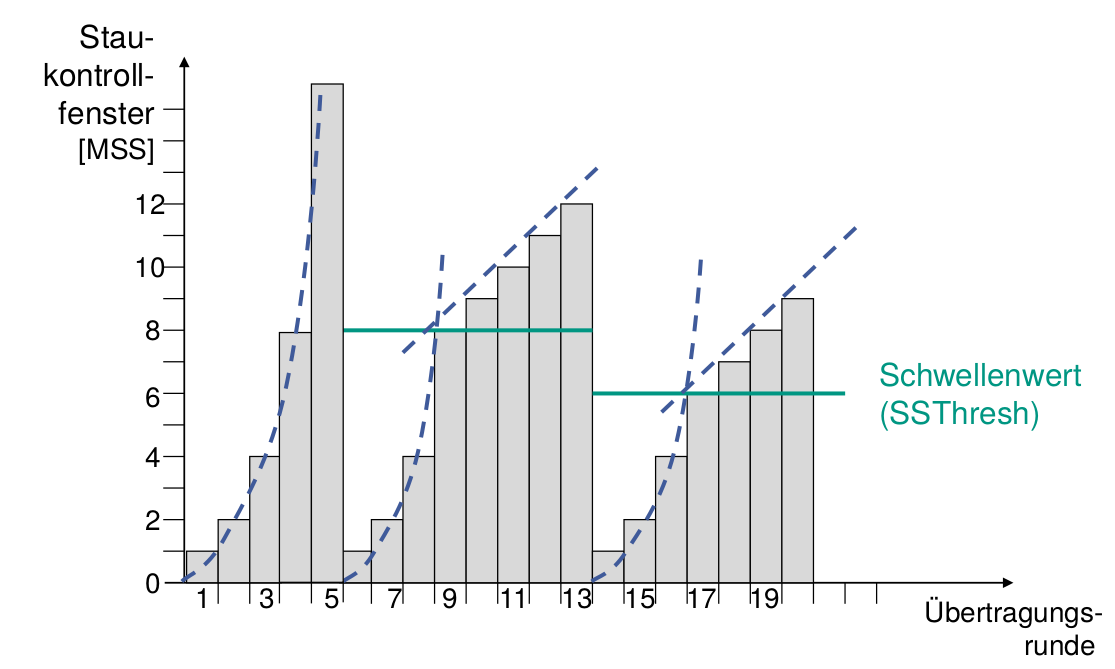
\includegraphics[width=0.33\textwidth]{TCPStaukontrolle}\end{figure}